\documentclass[12pt,a4paper]{article}
\usepackage[utf8]{inputenc}
\usepackage[english]{babel}
\usepackage{enumerate}
\usepackage{amsmath}
\usepackage{amsfonts}
\usepackage{amssymb}
\usepackage{graphicx}
\usepackage{fourier}
\usepackage[left=2cm,right=2cm,top=2cm,bottom=2cm]{geometry}
\usepackage{commath}
\usepackage{cancel}
\usepackage{placeins}
\author{Juan Carlos Apitz, ID 012523821}
\title{STAT572 - Homework Assignment 1}
\begin{document}

\maketitle

\section*{Lab Exercise - Fisher Scoring on the Standard Normal:}
To implement this exercise we need to find the score vector and the information matrix of the normal distribution's log-likelihood function:\\
The score vector is:
$U(\vec{\theta})=\begin{bmatrix}
\dfrac{\partial \log \mathcal{L}}{\partial \mu} \\ 
\dfrac{\partial \log \mathcal{L}}{\partial \sigma^2} 
\end{bmatrix}=
\begin{bmatrix}
\dfrac{\sum_{i=1}^n x_i - n\mu}{\sigma^2} \\ 
\dfrac{-n}{2\sigma^2}+\dfrac{\sum_{i=1}^n(x_i-\mu)^2}{2(\sigma^2)^2} 
\end{bmatrix}$\\
The information matrix is: $I(\vec{\theta})=-E[H(\vec{\theta})]=
\begin{bmatrix}
\dfrac{n}{\sigma^2} & 0 \\ 
0 & \dfrac{n}{2(\sigma^2)^2} 
\end{bmatrix}$\\
The MLE estimate is given by $\hat{\theta}=\theta_0+I^{-1}(\vec{\theta})U(\vec{\theta})$

\subsection*{Code (see next page):}

The code below implements MLE estimation using the Fisher Scoring method on the normal distribution. For simplicity I chose the standard normal, i.e. $\mu=0$, $\sigma^2=1$.

\begin{figure}[ht!]
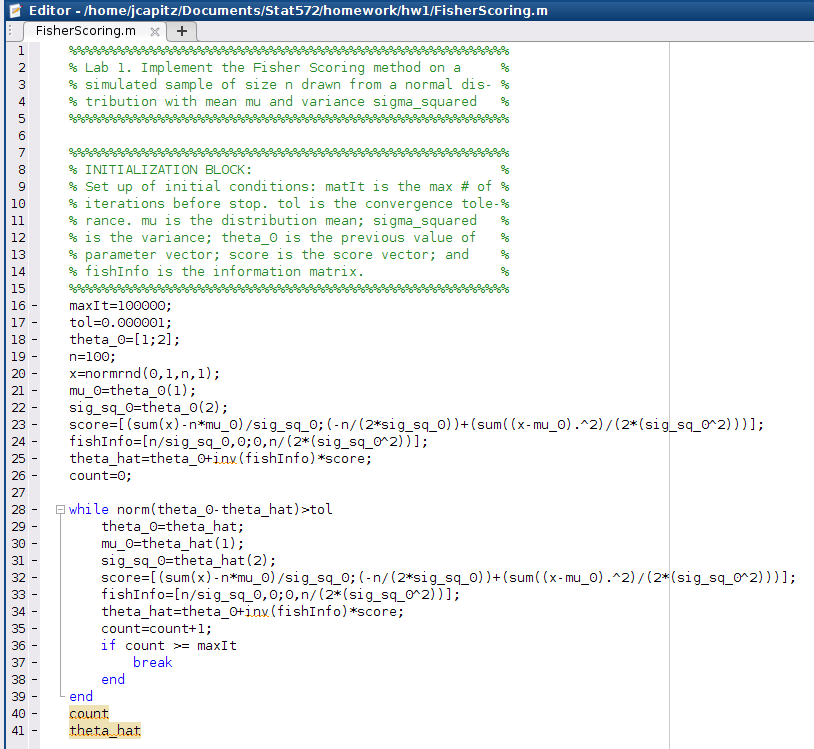
\includegraphics[scale=.60]{FisherScoringCode.png}
\caption{Code to implement MLE estimation on the standard normal distribution using Fisher Scoring.}
\label{fig1:lab}
\end{figure}

\FloatBarrier

\begin{figure}[ht!]
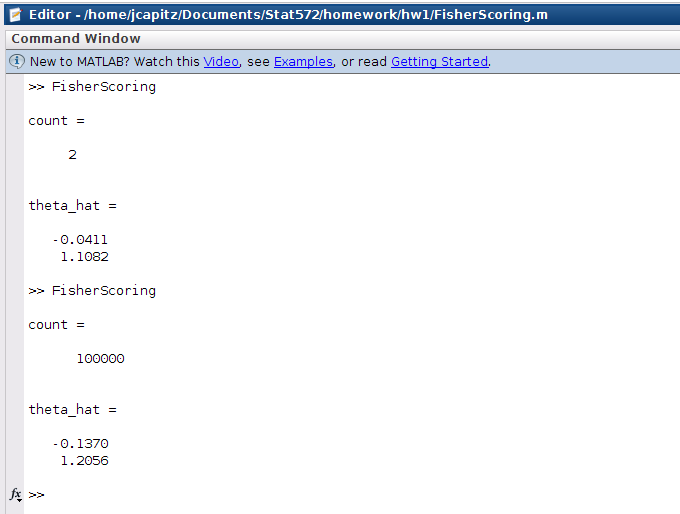
\includegraphics[scale=.70]{FisherScoringResult.png}
\caption{Results on implementing MLE estimation on the standard normal distribution using Fisher Scoring.}
\label{fig2:lab}
\end{figure}

As a trial I used $\mu_0=1$ and $\sigma^2_0=2$ to initialize the algorithm, set up the maximum number of trials to $100,000$ and the convergence tolerance to $0.000001$. The tolerance is compared to the value $||\hat{\theta}-\theta_0||$, a reasonable measure of vector distance between the vector $\hat{\theta}$ and $\vec{\theta_0}$. When the tolerance is applied, the algorithm converges in two iterations. I also let ran for $100,000$ iterations to see the results. It was interesting to observe that in the longer run the estimates were actually much worse than the two iteration run. The results are shown below with the first vector component of the MATLAB vector \textbf{theta\_hat} representing the mean, and the second component representing the variance.

\FloatBarrier



\section*{Exercise 2.1}

\begin{figure}[ht!]
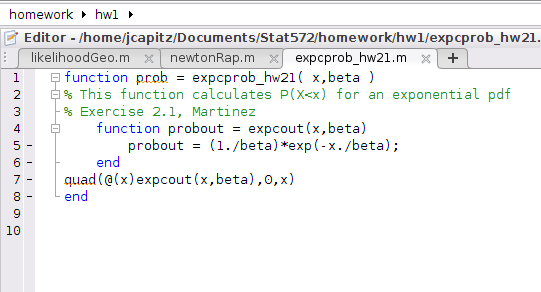
\includegraphics[scale=.70]{code_21.png}
\caption{Code to calculate $p(X<x_0)$ if $X\sim exp(\beta)$.}
\label{fig1:2.1}
\end{figure}

I wrote a short script to create a table that compares the results of the function from exercise 2.1 with the results of calculating $P(X<x_0)$ for the exponential function with $\beta=1$ using MATLAB's built-in function $expcdf(x,\beta)$. My function matches exactly the MATLAB results. See output below:

\begin{figure}[ht!]
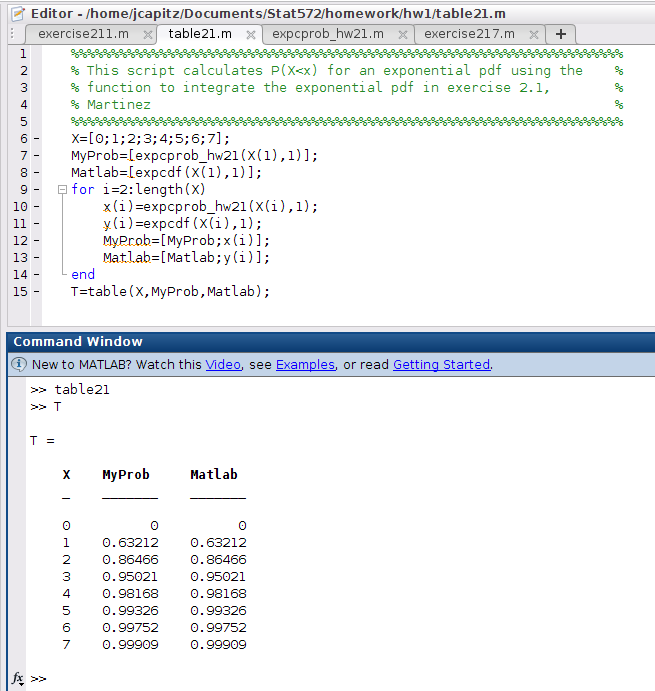
\includegraphics[scale=.70]{table21.png}
\caption{Table showing $p(X<x_0)$ for the exponential cdf using ex. 2.1 function and MATLAB's $expcdf(x,\beta)$.}
\label{fig2:2.1}
\end{figure}

\FloatBarrier

\section*{Exercise 2.2}

In this exercise I simply gave the above functions the input "inf", which in MATLAB it represents infinity. Since the support of the exponential pdf is $(0,\infty)$, the result below confirms that the function developed in ex. 2.1 actually integrates to 1. This confirms this canonical property of probability functions. In the case of the exponential pdf, we have $\displaystyle \int_0^\infty \dfrac{1}{\beta} e^{-\dfrac{x}{\beta}} \ dx=1$. The result is presented below.

\begin{figure}[ht!]
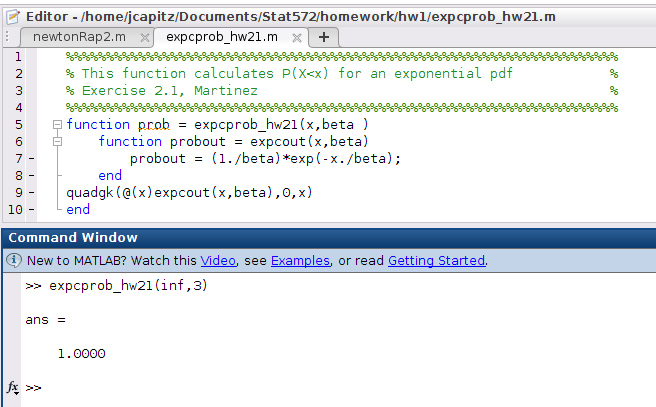
\includegraphics[scale=.70]{excersie22.png}
\caption{Code to calculate $p(0<X<\infty)$ if $X\sim exp(\beta=3)$.The result is 1.}
\label{fig1:2.2}
\end{figure}

\FloatBarrier

\section*{Exercise 2.11}

In this exercise we find the maximun for a normal pdf with $\mu=3, \ \sigma^2=1$ using the MATLAB function fminbnd(). This function actually find the $argmin f(x)$, thus the objective function has to be $-f(x)$. 

\begin{figure}[ht!]
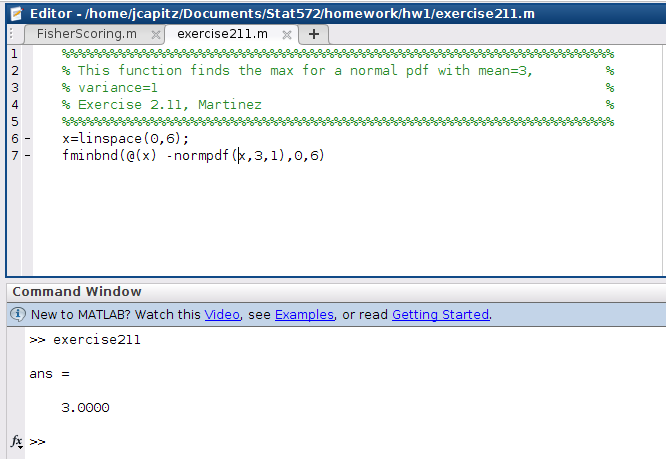
\includegraphics[scale=.70]{results211.png}
\caption{Code to calculate $argmax f(x)$ where $f(x)$ i.e. a normal distribution with $\mu=3,\ \sigma^2=1$.}
\label{fig1:2.11}
\end{figure}

\FloatBarrier

The code above implements this maximization with the result $argmax f(x)=3$. We know this is correct because this is the value of $\mu$ that is most likely for a probability distribution, i.e. this pdf reaches a maximum at the mean.

\section*{Exercise 2.17}

In this exercise we find $p(X<3)$ and $p(X>5)$ for a random variable $X\sim N(\mu=5,\ \sigma^2=4)$ using MATLAB's normspec() and normcdf(). 

\begin{figure}[ht!]
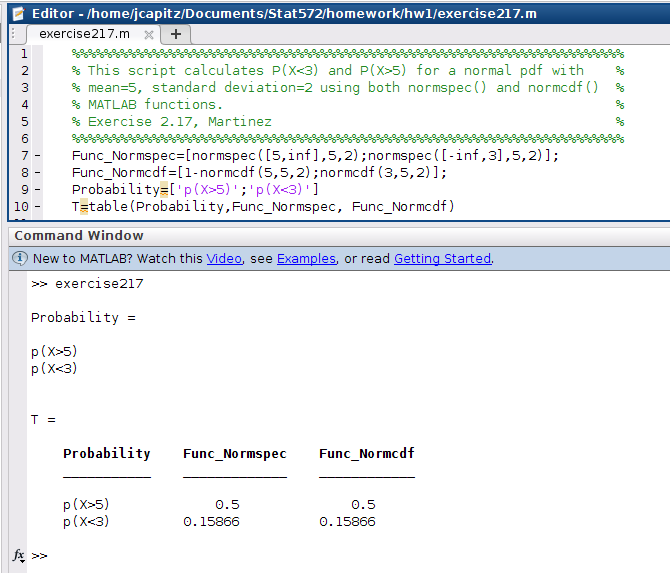
\includegraphics[scale=.70]{exercise217.png}
\caption{Code to calculate $p(X>5)$ and $p(X<3)$ using normspec() and normcdf().}
\label{fig1:2.17}
\end{figure}
\FloatBarrier

The above code computes the required probabilities and places the result on a MATLAB table for comparison. Both function results agree as expected, although to compute $p(X>5)$ we need to use the reciprocal probability calculation $1-normcdf(X,\mu,\sigma)$ since normcdf() only computes $p(X<x_0)$. For normspec() we can actually input $inf$ and get a result. In addition normspec() also provides a graphical output for this calculation. See figure \ref{fig2:2.17} and \ref{fig3:2.17} below.

\begin{figure}[ht!]
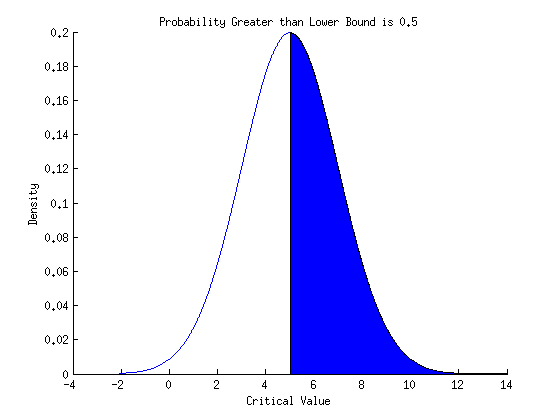
\includegraphics[scale=1]{greater_than_mean_217.png}
\caption{$p(X>5)$ using normspec().}
\label{fig2:2.17}
\end{figure}

\begin{figure}[ht!]
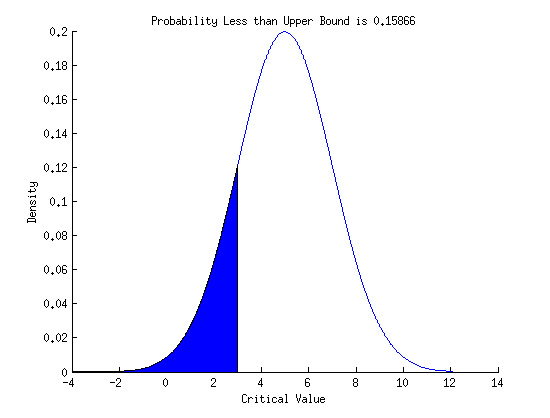
\includegraphics[scale=1]{less_than_x_217.png}
\caption{$p(X<3)$ using normspec().}
\label{fig3:2.17}
\end{figure}

\FloatBarrier


\end{document}